\chapter[Conclusions and Future Work]{Conclusions and Future Work}
\label{chap:Conclusions}

The research presented in this dissertation develops and evaluates tools that allow users to manage autonomy by managing information. This autonomy management approach is applied to the application domain of using a UAV to support Wilderness Search and Rescue. Autonomous components and autonomy management tools operate at three distinctive temporal scales, \textbf{strategic}, \textbf{between-episodes}, and \textbf{within-episode}. These scales represent three different temporal spans that are relevant to many problems: a long-term span that uses data and models from similar problems generates behavior that exploits common trends; a medium-term span that uses data and models obtained from prior attempts to solve the specific task to shape a new attempt to solve the problem; and a short-term span that uses real-time data and insights obtained from performing the task to shape the behavior of the autonomy moving forward, respectively. By managing two information representations, a \textit{probability distribution map} and a \textit{task-difficulty map}, at each temporal scale, the domain expert user becomes an ``intelligent sensor'', ``digesting'' information from various sources and then feeding the ``filtered'' information to the system in forms the system can understand. Doing so enables the user to influence the behavior of the autonomous subsystems without understanding the statistical models or complex algorithms used in the autonomous components.

%=====================================================================================================
\section{Conclusions}
\label{conclusions}

Challenges of integrating autonomy into an intelligent system can be characterized along two dimensions: \textit{attributes of an intelligent system} (capability, information management, performance evaluation) and \textit{organizational scale} (individual, collaborative agents, distributed system). These attributes can serve as a guideline when designing autonomous components and autonomy management tools. 

We proposed a new autonomy management approach where the user influenced the behavior of an autonomous system (or subsystem) by hierarchically managing information at different temporal scales through two information representations:  a \textit{probability distribution map} and a \textit{task-difficulty map}. We designed autonomous components and autonomy management tools for a wilderness search and rescue problem, and tailored the autonomy and tools so that they could operate across the different temporal scales.  We then presented evidence that these tools enabled the user to create and modify these maps by incorporating their domain knowledge and information. 

The key to making it possible for the autonomy algorithms to work across temporal scales was to endow them with the ability to use the information provided by the human to create real-time plans.  These plans were then presented to the human, allowing him or her to modify the plan by modifying the type of information provided to the planner.  For the wilderness search and rescue problem, this required the creation of multiple real-time UAV-based path planning algorithms that used the maps as input.  

Human-interaction with the path planners came in two forms: modifying the maps and providing constraints on the autonomy. The maps are consistent with a Bayesian approach to decision making, yielding algorithms that outperform the state-of-the-art approaches for problems that require real-time feedback and support partial object detection.  Constraints were implemented using a sliding autonomy interface where the user influenced the planner by specifying path segment endpoint constraints (spatial) and flight segment durations (temporal).

A user study provided evidence that this autonomy management approach enabled the human-autonomy team to outperform the human or autonomy working alone.  Additionally, the user study provided evidence that this performance increase was accompanied by a reduction in human cognitive workload and an improvement in the human's perception of the human-automation experience.



Then when these maps are used for UAV path planning, we developed multiple Intelligent Path Planning Algorithms that support real-time feedback and partial detection, and propose a sliding autonomy interface where the user can manage path planning autonomy by managing path segment endpoint constraints (spatial) and flight duration (temporal). We demonstrate the usefulness of this autonomy management approach and results from a user study show that this approach enables the human-autonomy team to outperform human or autonomy working alone, reduces the human's cognitive workload, and improves the human experience in the human-autonomy interaction.

%=====================================================================================================
\section{Contributions}
\label{contributions}

This dissertation has the following main contributions to Computer Science research.

\begin{itemize}
\item We identified autonomy integration challenges along two dimensions. These requirements served as a guideline in our design of the autonomous components and autonomy management tools in our proposed solution.
\item We propose a new autonomy management approach: managing autonomy by hierarchically managing information at three temporal scales through two information representations: a \textit{probability distribution map} and a \textit{task-difficulty map}. We developed various autonomous components and autonomy management tools at each temporal scale and demonstrated the usefulness of the approach.
\item We designed a Bayesian model that uses terrain features and past human behavior data to model lost-person behaviors. The user can influence the probability distribution map generated by changing prior beliefs and by selecting what subset of past human behavior data to feed to the model.
\item We designed two autonomy management tools that enable the user to manage the \textit{probability distribution map} and \textit{task-difficulty map} by mouse and finger gestures.
\item We proposed a heuristic, \textit{Mode Goodness Ratio}, which uses a Gaussian Mixture Model to prioritize search subregions, and enables a hierarchically search for effective paths through the parameter space at different levels of resolution.
\item We designed multiple path planning algorithms that support partial detection. We evaluated the performance of these algorithms against state-of-the-art algorithms using three real WiSAR scenarios and show that our algorithms generate near-optimal paths in real-time.
\item We proposed the Sliding Autonomy Interface that enables the user to manage path planning autonomy along two dimensions: constraints (spatial) and flight duration (temporal). Data from a user study show that this approach enables the human-autonomy team to outperform human or autonomy working alone, reduces the human's cognitive workload, and improves the human experience in the human-autonomy interaction.
\end{itemize}

%=====================================================================================================
\section{Future Work}
\label{futurework}

This section presents a few of the natural extensions from current research that can be pursued as future work. We list them in the order of the three temporal scales and show how they relate to the various components of the dissertation work (see Figure~\ref{ProjectComponents2}).

\begin{figure}
\centering
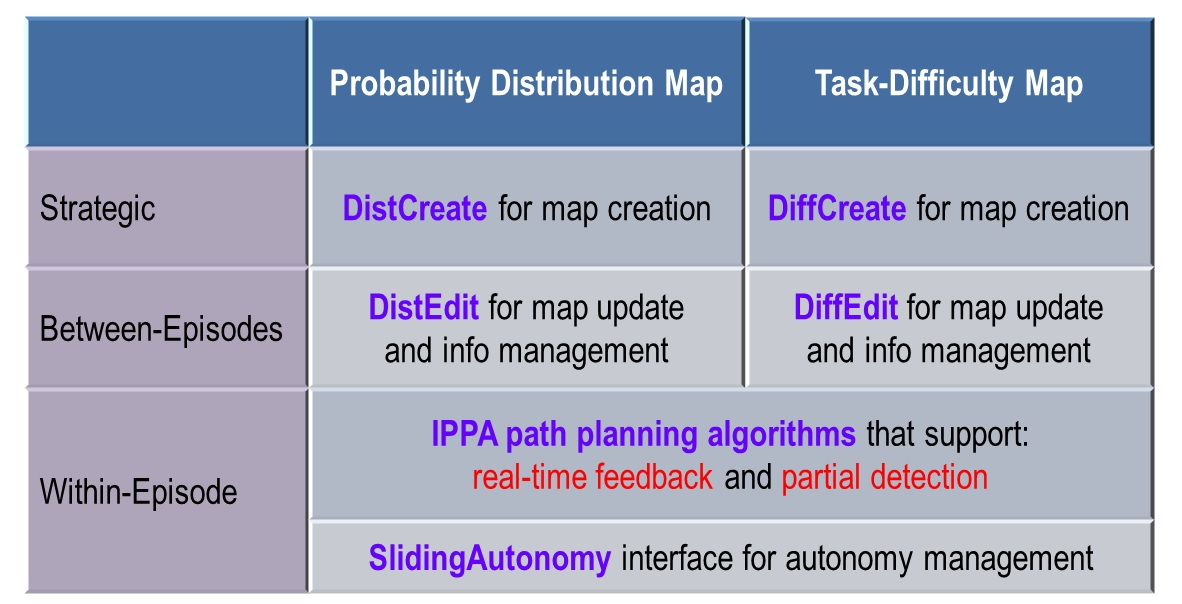
\includegraphics[width=6in]{ProjectComponents.JPG}
\caption{Autonomous components and autonomy management tools of the dissertation work at each temporal scale/hierarchy.}
\label{ProjectComponents2}
\end{figure}

%===================================================
\subsection{At the Strategic Scale}

Presently, the \textbf{DistCreate} component uses a set of default prior belief parameters (transitional probabilities between pairs of terrain features) that can be changed by the domain expert user based on his her her domain expertise and information only the user can interpret. It would be beneficial if the system could automatically suggest transitional probability values based on statistics from past incidents~\cite{Koester2008Lost} after the user provides some initial lost person profile information (such as age, gender, profession, etc.). When the user wants to modify the suggested parameters, instead of typing in values, it would be helpful to provide a tool that allows the user to visually see the prior belief distributions. By moving two sliders to change the mean and standard deviation values, the user could see how the shapes of the distributions changes. Ideally, the user could also see how this affects the shapes of the final prior / posterior predictive probability distributions with instant feedback. This immediate visual feedback would allow the user to understand causal effects and therefore help the user form a mental model of the system that is similar to how the system truly works. Figure~\ref{Mockup1} shows a mock up screen of such a tool. Computationally, instant feedback would require that we perform complex matrix computations on the GPU using CUDA (Compute Unified Device Architecture) architecture. To evaluate how this would affect the human-autonomy interaction and the performance of the human-autonomy team, a user study could be performed.

\begin{figure}
\centering
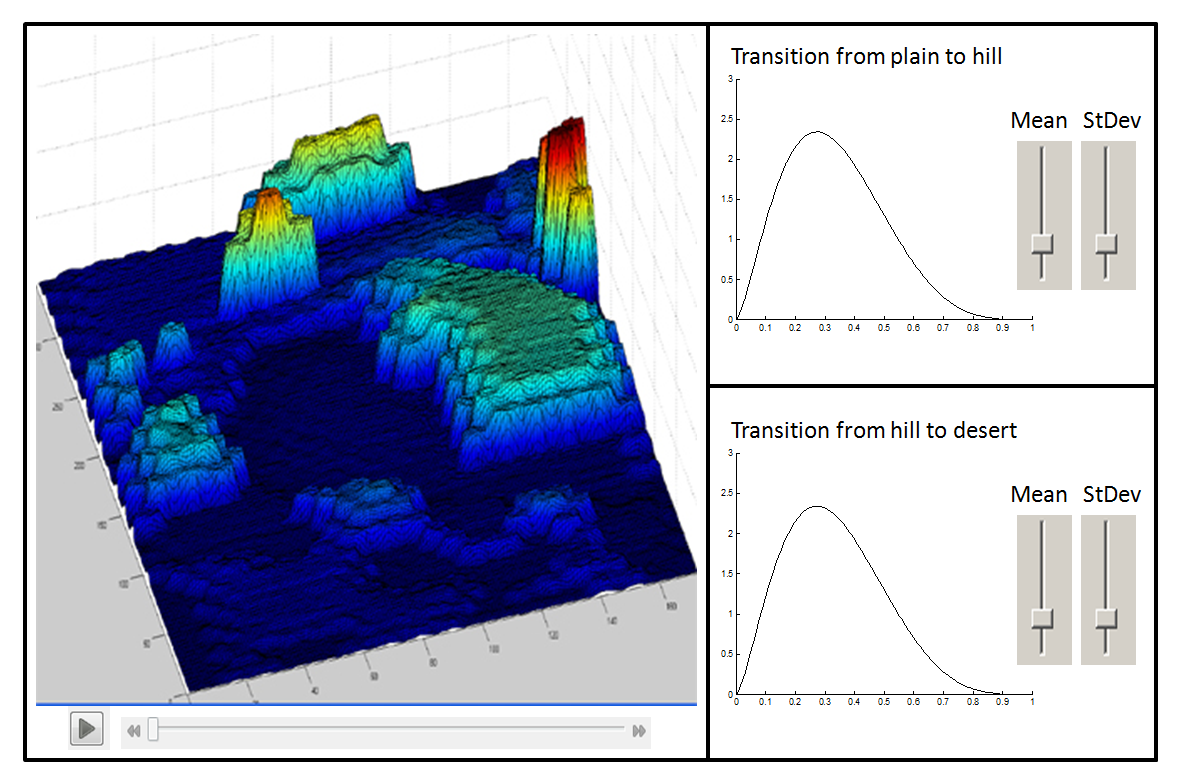
\includegraphics[width=6in]{Mockup1.png}
\caption{A mock up screen for the management tool interface at the strategic scale.}
\label{Mockup1}
\end{figure}

The \textbf{DistCreate} component considers three terrain features: topography, elevation, and vegetation density. It is probably beneficial to incorporate more factors that affect lost-person behaviors into the network. Such factors include but are not limited to direction of travel, trail following, missing person profile, panicking factor, weather conditions and season of the year. Such factors could be easily included into the existing Bayesian network as prior nodes. Additional utility tools might be needed to generate geographic data when it is not directly available. For example, if trail data cannot be automatically extrapolated, such utility tools would allow the search to manually mark trails on a map.

Currently the user can only specify whether to use past-human behavior data or not with the \textbf{DistCreate} component. In the future, as more past-human behavior data become available, the data could be stored in a database, and the user could further decide which subset of the behavior data to use by querying the database. For example, the user could choose to only use data of the same search region, season of the year, or only data from people who have simililar profile (age, gender, profession, etc.) with the missing person.

The \textbf{DiffCreate} component uses vegetation coverage data from USGS satellite imagery data to extrapolate vegetation density and determines task difficulty (detection probably). A more advanced model could be designed to include additional factors such as UAV height above ground, time of the day, season of the year, ``seeability''~\cite{Morse2010UAV}, and sensor specific properties (e.g., an infrared multi-spectrum camera). Additional constraints such as no-fly zone or dangerous areas could also be included in the \textit{task-difficulty map}.

%===================================================
\subsection{At the Between-Episodes Scale}

The \textbf{DistEdit} and \textbf{DiffEdit} components at this temporal scale let the user use mouse and finger gestures to edit the \textit{probability distribution map} and the \textit{task-difficulty map} generated from the strategic scale in a 3D environment. In this dissertation we only validated the usefulness of these two tools by demonstration. To better evaluate the usefulness of the two tools, a well-designed user study should be performed. Ideally, these tools should be given to real search and rescuers to generate maps for real WiSAR scenarios. The user should be able to modify these maps as new information becomes available. For example, the maps should be modified when a piece of clothing or candy wrapper is found during the search, or when ground searchers have thoroughly searched an area and confirmed that the missing person is unlikely located at certain regions. These tools could also be integrated with the Sliding Autonomy component so the two maps can be updated in real time while the UAV is in the air during the mission.

%===================================================
\subsection{At the Within-Episode Scale}

At this temporal scale we designed multiple intelligent path planning algorithms that support real-time feedback and partial detection. These algorithms assume the missing person is stationary and the probability distribution map and the task-difficulty map are static. Because these algorithms are very fast, they should be improved to deal with moving targets, changing probability distributions and a task-difficulty map that changes over time. Then to further expand the problem, these algorithms could be improved to work with multiple targets or support multiple UAVs. We leave these to future work.

The \textbf{SlidingAutonomy} interface allows the user to affect the behavior of the path planning autonomy by setting temporal and spatial constraints. The user study we performed was a short-term study where each user had only minimal training before using this interface. Because a human's trust in autonomy can change over time, it would be interesting to research how the user's trust gets calibrated when the user uses this autonomy management approach for a long period of time. Would the user be able to gradually identify the weaknesses of the path planning autonomy and remedy correctly? Would the user overtrust autonomy and perform worse in the long run? Or would the user undertrust autonomy because autonomy makes obvious mistakes in certain scenarios? In our user study, the two scenarios used are both relatively easy scenarios. When a more complicated \textit{probability distribution map} and \textit{task-difficulty map} are used, the benefit of using the \textbf{Sliding Autonomy} interface might be more obvious, and it would interesting to investigate how users would react to that. It is also possible to let the user specify the number of top regions through the \textbf{Sliding Autonomy} interface for the Top2 and TopN algorithms and see how that would affect the human-autonomy interaction. These questions can only be answered with a long-term user study, which we leave for future work.

At this temporal scale, while the UAV is in the air during mission, as information is collected and processed by the collective search and rescue team, situation could arise when the \textit{probability distribution map} and/or the \textit{task-difficulty map} become incorrect. If these two maps cannot be updated in real-time, how could the user use the \textbf{SlidingAutonomy} interface to influence path planning autonomy in order to address the information change? The user might want the UAV to avoid certain regions or force the UAV to visit other regions repeatedly. How well does the \textbf{SlidingAutonomy} interface support such interaction could be another interesting research topic. A user study could be performed to evaluate the human-autonomy interaction experience and the performance of this Sliding Autonomy approach.


%===================================================
\subsection{The Overall Autonomy Management Approach}

In this dissertation we applied the proposed autonomy management approach to the application domain of using a UAV to support Wilderness Search and Rescue. It is worth hypothesizing that this approach could be generalized and applied to many application domains. For example, when using an assistive robot to help a therapist treat children with autism, robot autonomy could also be managed by hierarchically managing information at different temporal scales. 

At the \textbf{strategic} scale, before a child with autism begins clinical treatments, the therapist performs a series of evaluations. Information collected is analyzed to determine the deficiencies, then a treatment plan is created identifying areas the therapist should focus on (e.g., joint attention, turn taking). Here this 
\textit{areas of focus} map is analogous to the \textit{probability distribution map} we discussed before. It is possible to develop a model to assist the therapist in generating this initial plan at the general trend scale. The therapist could decide what model parameters and dataset to use to train the model or to affect the plan. Similarly, a \textit{task-difficulty map} could be created identifying areas where the therapy treatment might not be very effective.

At the \textbf{between-episodes} scale, a child with autism may receive one or two treatments each week. At different stages of the treatment the therapist might focus on different areas or reinforce certain behaviors in each session. The therapist may prefer the robot to have exaggerated facial expression and movement in one session but appear calmer and more verbose in another; or the therapist might want the robot to demonstrate a higher degree of reliance on the therapist. Ideally, by adjusting the areas of focus and the task-difficulty map at the between-sessions scale, the therapist could take advantage of special knowledge or experience and indirectly affect the robot's autonomous behaviors by managing what information to provide.

At the \textbf{within-episode} scale, during a clinical session a child with autism might not behave as the therapist expects (due to fatigue, previous events, or unexpected events). The therapist needs to be able to manage the robot's autonomous behaviors in real-time in order to improve or maximize the potentials of the treatment. The ability to modify the areas of focus and the task-difficulty map in real time affords the therapist the desired levels of control. The therapist could also strategically plan out the order of activities (targeted to different deficiencies) and desired intensity (time allocated to each activity) during the session to improve the efficiency of the treatment. At the within-session scale, the therapist is really actively collecting information (the child's behavior and reaction), digesting the information, and then deciding what information to provide to the system, in forms the system can understand, in order to manage the autonomous behavior of the robot.

Applying our proposed autonomy management approach to a completely different application domain and then evaluating how well the approach generalized is an important part of future work.